\documentclass[10pt,a4paper]{article}

\usepackage{marktwo}
\usepackage{graphicx}

\begin{document}

\makemathtitle
    {Reflection and Refraction}
    {Introduction to the laws of reflection and refraction in linear dielectrics}
    {Vivek Kalita}
    {Department of Physics, IISER Mohali}
    {10 November 2026}

\tableofcontents

\section{Maxwell's equations and the boundary conditions}



Let's start with the Maxwell's equations:
\begin{axiom}[Maxwell's equations]

The four fundamental equations for the electromagnetic field are

\[
\begin{array}{rcl@{\qquad}l@{\qquad\qquad}rcl@{\qquad}l}
\displaystyle
\iint_{\partial V}\mathbf{D}\cdot\mathrm{d}\mathbf{A}
&=&
\displaystyle\iiint_V\rho_f\,\mathrm{d}V
&\text{(A1)}
&
\displaystyle
\oint_{\partial S}\mathbf{E}\cdot\mathrm{d}\mathbf{l}
&=&
\displaystyle-\frac{\mathrm{d}}{\mathrm{d}t}
\iint_S\mathbf{B}\cdot\mathrm{d}\mathbf{A}
&\text{(A2)}
\\[1.2em]
\displaystyle
\iint_{\partial V}\mathbf{B}\cdot\mathrm{d}\mathbf{A}
&=&0
&\text{(A3)}
&
\displaystyle
\oint_{\partial S}\mathbf{H}\cdot\mathrm{d}\mathbf{l}
&=&
\displaystyle
\iint_S\mathbf{J}_f\cdot\mathrm{d}\mathbf{A}
+\frac{\mathrm{d}}{\mathrm{d}t}
\iint_S\mathbf{D}\cdot\mathrm{d}\mathbf{A}
&\text{(A4)}
\end{array}
\]

The constitutive relations are

\[
\mathbf{D}=\varepsilon_0\mathbf{E}+\mathbf{P}
\qquad
\mathbf{H}=\frac{\mathbf{B}}{\mu_0}-\mathbf{M}.
\]

\end{axiom}






\subsection{Boundary conditions at a medium-discontinuity}
\begin{figure}[H]
    \centering
    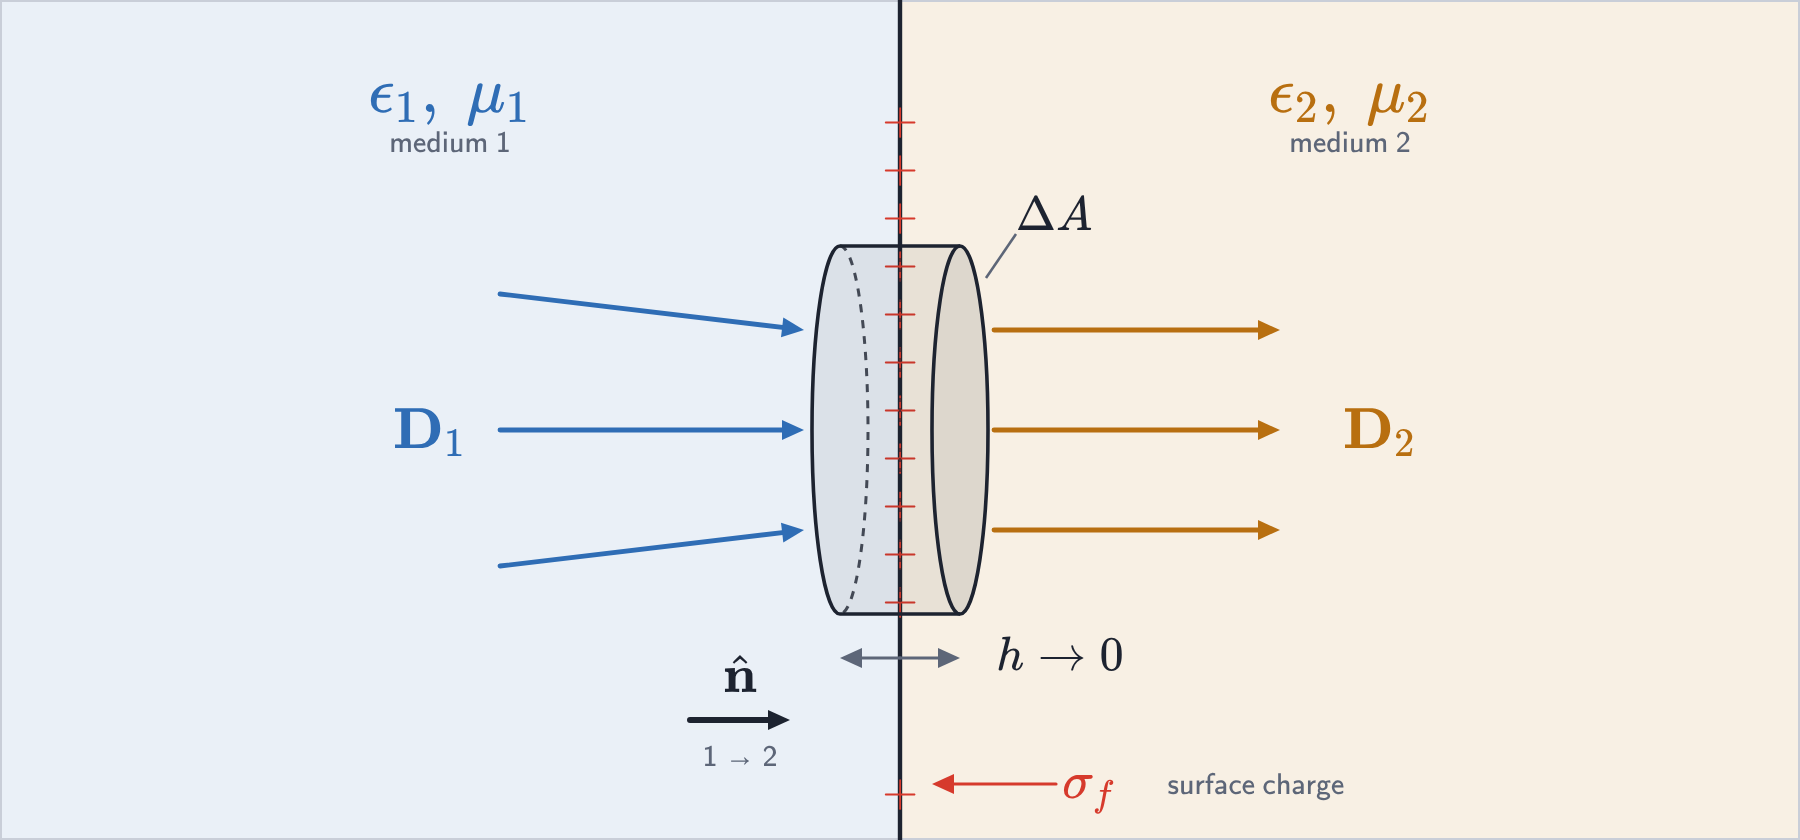
\includegraphics[width=0.70\textwidth]{images_reflection_refraction/pillbox.png}
    \caption{The Gaussian pillpox}
\end{figure}
\begin{enumerate}
    \item As illustrated in the figure, consider a Gaussian pillbox of cross-sectional
    area \(A\) and height \(h\) at the interface between media 1 and 2.
    Let \(\mathbf{n}\) be the unit normal directed from medium 1 to medium 2.
 By Gauss's law for the electric displacement field,
    \[
        \oint_{\partial V} \mathbf{D}\cdot d\mathbf{a}
        = Q_{f,\mathrm{enc}}
        = \sigma_f A ,
    \]
 thus,
    \[
        \mathbf{n}\cdot(\mathbf{D}_2-\mathbf{D}_1)=\sigma_f .
    \]

\item    Applying Gauss's law for the magnetic flux density to the same pillbox gives
    \[
        \oint_{\partial V} \mathbf{B}\cdot d\mathbf{a}=0
        \quad\Longrightarrow\quad
        \mathbf{n}\cdot(\mathbf{B}_2-\mathbf{B}_1)=0 .
    \]
\end{enumerate}

\begin{figure}[H]
    \centering
    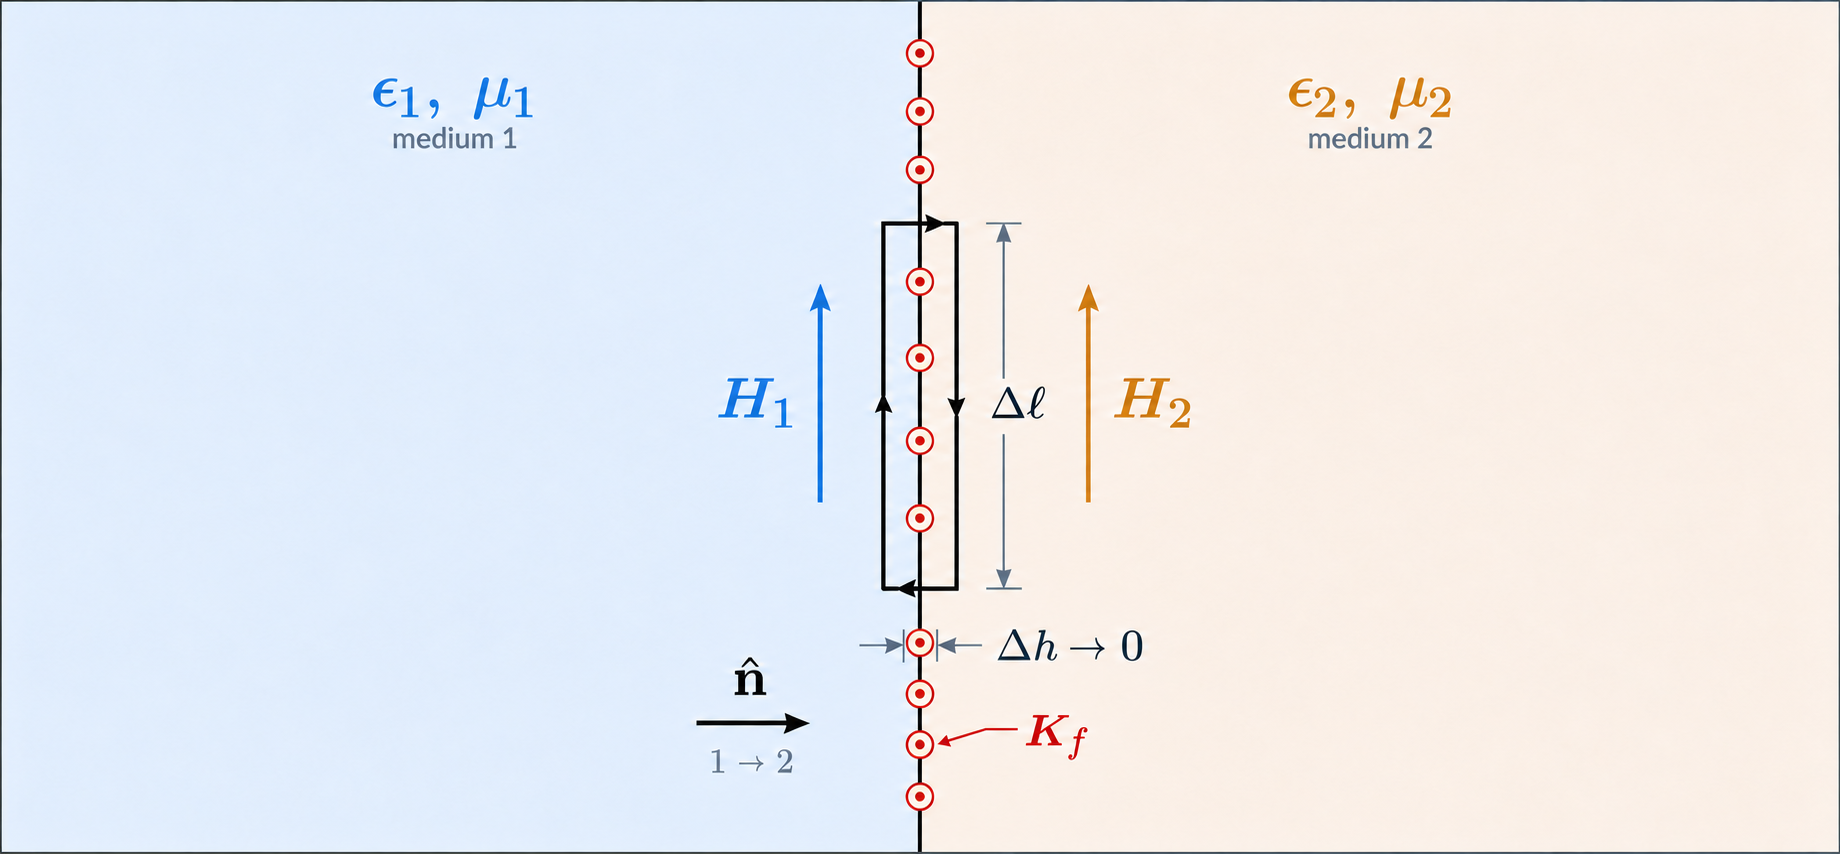
\includegraphics[width=0.7\textwidth]{images_reflection_refraction/loop.png}
    \caption{The amperian loops}
\end{figure}
\begin{enumerate}
    \item 
    Consider an infinitesimal rectangular loop on the interface. We have:
    \[
        \oint_C \mathbf{E}\cdot d\boldsymbol{\ell}
        =
        -\frac{d}{dt}\int_S \mathbf{B}\cdot d\mathbf{a}.
    \]
    As the loop height tends to zero, the magnetic flux through its area
    vanishes. So the tangential component of the electric field is continuous:
    \[
        \mathbf{n}\times(\mathbf{E}_2-\mathbf{E}_1)=\mathbf{0}.
    \]

    \item 
    Applying the Ampère--Maxwell law to the same loop gives
    \[
        \oint_C \mathbf{H}\cdot d\boldsymbol{\ell}
        =
        I_{f,\mathrm{enc}}
        +\frac{d}{dt}\int_S \mathbf{D}\cdot d\mathbf{a}.
    \]
    As the loop height tends to zero, the displacement-flux term vanishes:
    \[
        \mathbf{n}\times(\mathbf{H}_2-\mathbf{H}_1)=\mathbf{K}_{s,f}.
    \]
\end{enumerate}



\begin{theorem}[Boundary conditions for discontinuous media]
Let \(\mathbf{n}\) be the unit normal directed from medium 1 to medium 2.
The boundary conditions are
\[
\begin{aligned}
\mathbf{n}\times(\mathbf{E}_2-\mathbf{E}_1) &= \mathbf{0},
&\qquad
\mathbf{n}\times(\mathbf{H}_2-\mathbf{H}_1) &= \mathbf{K}_f,\\
\mathbf{n}\cdot(\mathbf{D}_2-\mathbf{D}_1) &= \sigma_f,
&\qquad
\mathbf{n}\cdot(\mathbf{B}_2-\mathbf{B}_1) &= 0.
\end{aligned}
\]
\end{theorem}

\begin{corollary}[Boundary conditions for linear isotropic media]
For \textnormal{\textcolor{red!70!black}{\textsf{linear, isotropic media}}},
\[
\mathbf{D}=\varepsilon\mathbf{E},
\qquad
\mathbf{B}=\mu\mathbf{H}.
\]
Therefore, at the interface,
\[
\begin{aligned}
\mathbf{n}\times(\mathbf{E}_2-\mathbf{E}_1) &= \mathbf{0},
&\qquad
\mathbf{n}\times\left(\frac{\mathbf{B}_2}{\mu_2}
-\frac{\mathbf{B}_1}{\mu_1}\right) &= \mathbf{K}_f,\\
\mathbf{n}\cdot(\varepsilon_2\mathbf{E}_2-\varepsilon_1\mathbf{E}_1)
&= \sigma_f,
&\qquad
\mathbf{n}\cdot(\mathbf{B}_2-\mathbf{B}_1) &= 0.
\end{aligned}
\]
If there is no free surface current or surface charge density, the boundary
conditions reduce to
\[
\begin{aligned}
E_{2\parallel} &= E_{1\parallel},
&\qquad
\frac{B_{2\parallel}}{\mu_2} &= \frac{B_{1\parallel}}{\mu_1},\\
\varepsilon_2 E_{2\perp} &= \varepsilon_1 E_{1\perp},
&\qquad
B_{2\perp} &= B_{1\perp}.
\end{aligned}
\]
\end{corollary}

\section{Plane Waves}
Consider a plane wave of the form
\[
\mathbf{E}(\mathbf{r},t)
= \mathbf{E}_0 e^{i(\mathbf{k}\cdot\mathbf{r}-\omega t)}.
\]
From Faraday's law we could relate the electric and the magnetic field as:
\[
\nabla\times\mathbf{E}
= -\frac{\partial\mathbf{B}}{\partial t}
\quad\Longrightarrow\quad
\mathbf{B}
= \frac{1}{\omega}\,\mathbf{k}\times\mathbf{E}.
\]
\begin{figure}[H]
    \centering
    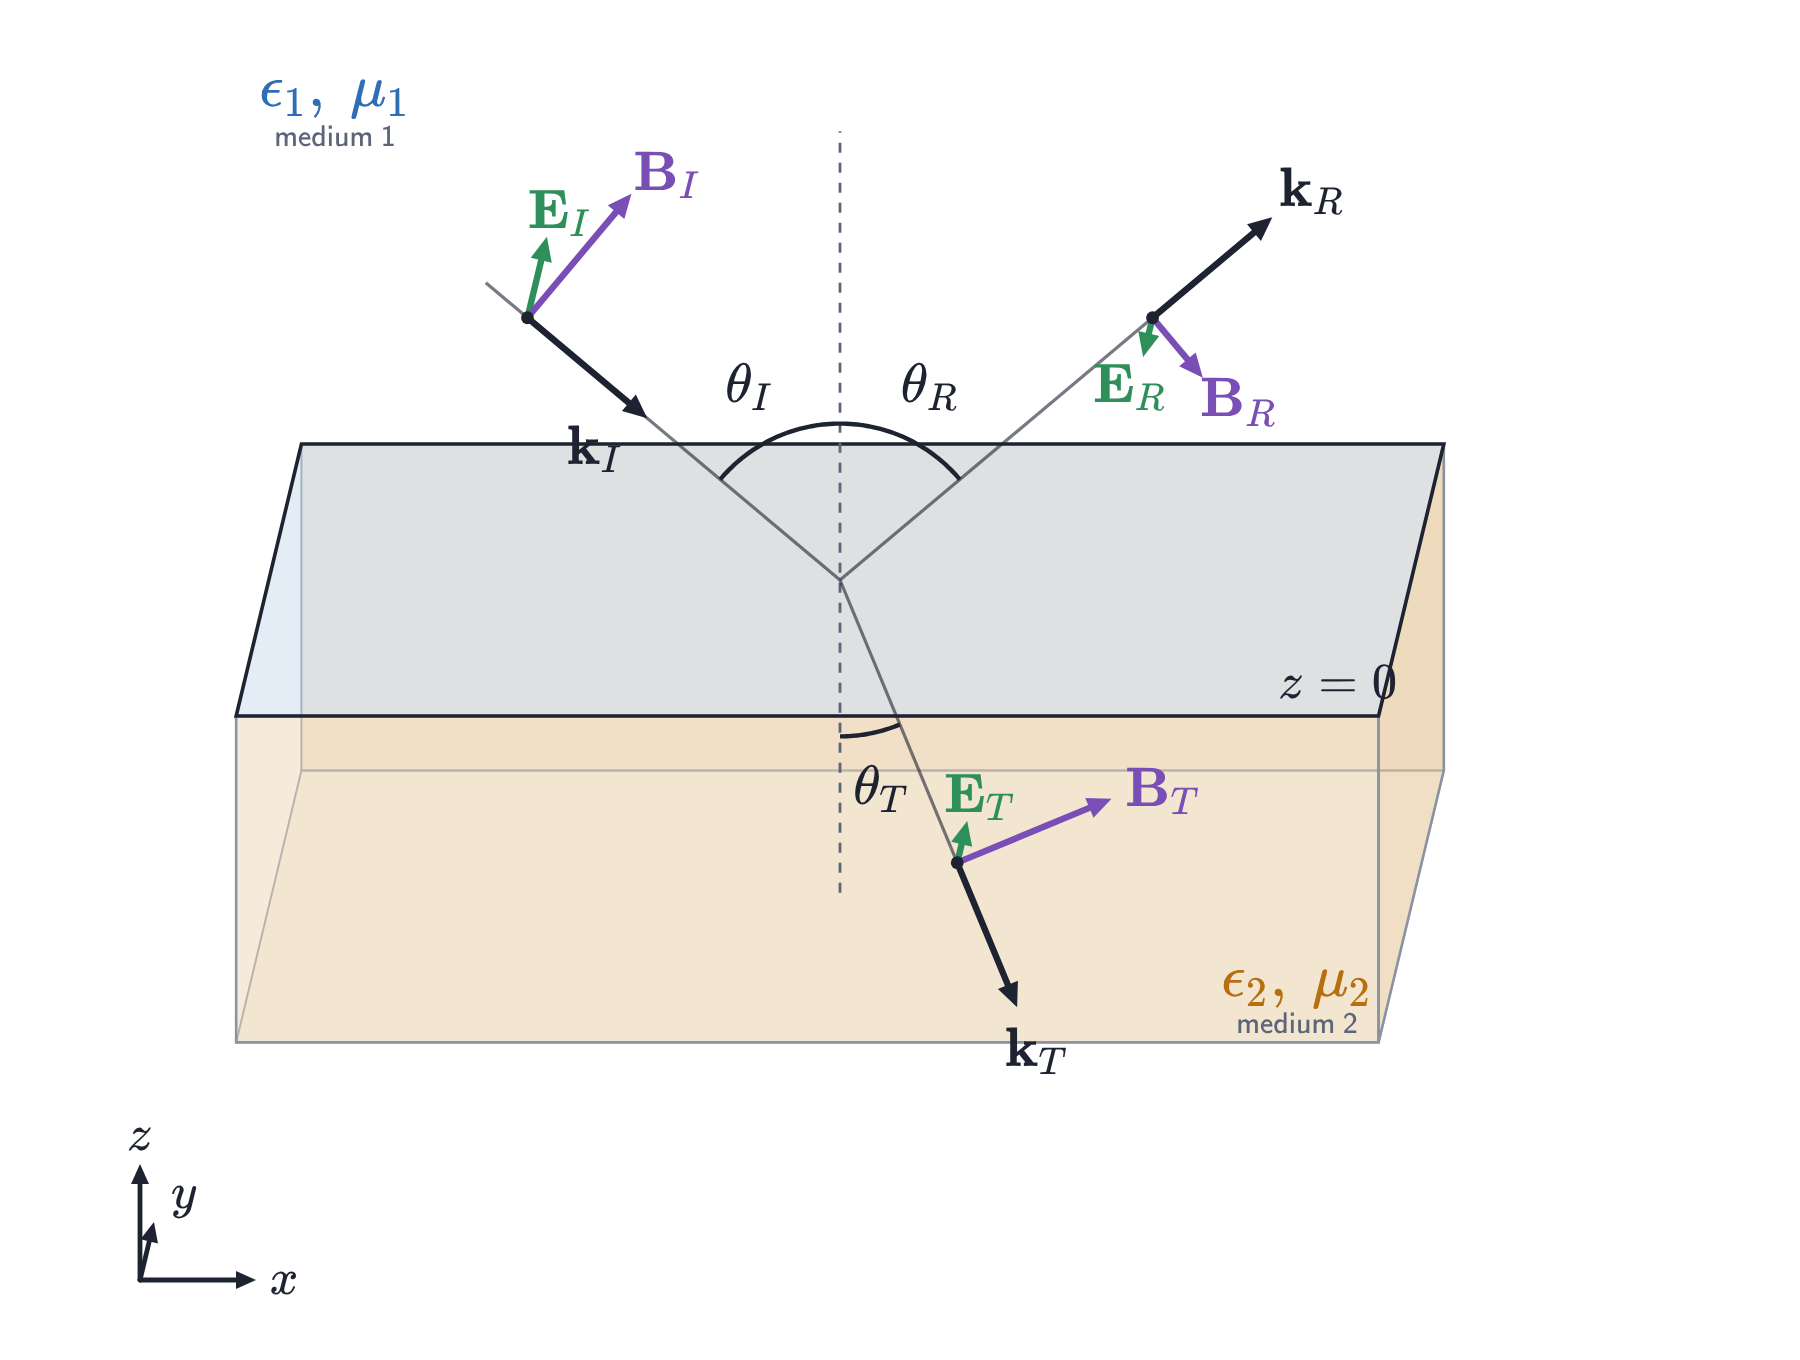
\includegraphics[width=0.7\textwidth]{images_reflection_refraction/reflection_incidence.png}
    \caption{A plane wave incident on a surface (the \(xy\) plane). Note that the wave is \(s\)-polarised, i.e. the electric field is parallel to the surface of incidence.}
\end{figure}

Let the wave vectors for the incident, reflected, and transmitted waves be
\[
\mathbf{k}_i
= k_1\left(\sin\theta_i\,\hat{\mathbf{x}}
          -\cos\theta_i\,\hat{\mathbf{z}}\right)
\quad
\mathbf{k}_r
= k_1\left(\sin\theta_r\,\hat{\mathbf{x}}
          +\cos\theta_r\,\hat{\mathbf{z}}\right),
\tag{\textsf{medium 1}}
\]
\[
\mathbf{k}_t
= k_2\left(\sin\theta_t\,\hat{\mathbf{x}}
          -\cos\theta_t\,\hat{\mathbf{z}}\right).
\tag{\textsf{medium 2}}
\]
Assume the electric fields are polarized along the \(y\)-axis:
\[
\mathbf{E}_i(\mathbf{r},t)
= E_0\hat{\mathbf{y}}\,
   e^{i(\mathbf{k}_i\cdot\mathbf{r}-\omega t)}
\quad
\mathbf{E}_r(\mathbf{r},t)
= E_{r0}\hat{\mathbf{y}}\,
   e^{i(\mathbf{k}_r\cdot\mathbf{r}-\omega t)},
\tag{\textsf{medium 1}}
\]
\[
\mathbf{E}_t(\mathbf{r},t)
= E_{t0}\hat{\mathbf{y}}\,
   e^{i(\mathbf{k}_t\cdot\mathbf{r}-\omega t)}.
\tag{\textsf{medium 2}}
\]
Using the relation between the magnetic field and the electric field:
\[
\mathbf{B}_i(\mathbf{r},t)
= \frac{k_1E_0}{\omega}
   \left(\cos\theta_i\,\hat{\mathbf{x}}
        +\sin\theta_i\,\hat{\mathbf{z}}\right)
   e^{i(\mathbf{k}_i\cdot\mathbf{r}-\omega t)}
\quad
\mathbf{B}_r(\mathbf{r},t)
= \frac{k_1E_{r0}}{\omega}
   \left(-\cos\theta_r\,\hat{\mathbf{x}}
        +\sin\theta_r\,\hat{\mathbf{z}}\right)
   e^{i(\mathbf{k}_r\cdot\mathbf{r}-\omega t)}
\tag{\textsf{medium 1}}
\]
\[
\mathbf{B}_t(\mathbf{r},t)
= \frac{k_2E_{t0}}{\omega}
   \left(\cos\theta_t\,\hat{\mathbf{x}}
        +\sin\theta_t\,\hat{\mathbf{z}}\right)
   e^{i(\mathbf{k}_t\cdot\mathbf{r}-\omega t)}.
\tag{\textsf{medium 2}}
\]

\subsection{Laws of reflection andd refraction}
At the interface \(z=0\), continuity of the tangential electric field gives
\[
E_{i\parallel}+E_{r\parallel}=E_{t\parallel}.
\]
Since all three electric fields are polarized along the \(y\)-axis, this becomes
\[
E_0 e^{i(k_1\sin\theta_i\,x-\omega t)}
+
E_{r0} e^{i(k_1\sin\theta_r\,x-\omega t)}
=
E_{t0} e^{i(k_2\sin\theta_t\,x-\omega t)}.
\]

\begin{enumerate}
    \item Since the boundary condition must hold for every \(x\), and all
    three waves have the same frequency, their tangential phase components
    must match:
    \[
        k_1\sin\theta_i
        =
        k_1\sin\theta_r
        =
        k_2\sin\theta_t.
    \]
    The first equality gives
    \[
        \theta_i=\theta_r,
    \]
    which is the \textcolor{red!70!black}{\textsf{law of reflection}}.

    \item The second equality gives
    \[
        k_1\sin\theta_i=k_2\sin\theta_t.
    \]
    For a plane wave in a
    \textcolor{red!70!black}{\textsf{homogeneous isotropic medium}},
    \[
        k_j=\frac{n_j\omega}{c}.
    \]
    where \(n_j\) is the refractive index. Since the frequency is the same in both media, this becomes
    \[
        n_1\sin\theta_i=n_2\sin\theta_t,
    \]
    which is Snell's law.
\end{enumerate}

\begin{theorem}[Law of reflection and Snell's law]
\begin{enumerate}
    \item According to the \textnormal{\textcolor{red!70!black}{\textsf{law of reflection}}},
    if \(\theta_i\) and \(\theta_r\) are the angles of incidence and reflection,
    respectively, then
    \[
        \theta_i=\theta_r.
    \]

    \item For an interface between two media with refractive indices \(n_1\)
    and \(n_2\), \textnormal{\textcolor{red!70!black}{\textsf{Snell's law}}} is
    \[
        n_1\sin\theta_i=n_2\sin\theta_t,
    \]
    where \(\theta_i\) and \(\theta_t\) are the angles of incidence and
    refraction, respectively.
\end{enumerate}
\end{theorem}

\subsection{Fresnel's equations}
At \(z=0\), continuity of the tangential electric field gives
\[
E_0+E_{r0}=E_{t0}.
\]
Continuity of the tangential magnetic field gives
\[
\frac{k_1\cos\theta_i}{\omega\mu_1}E_0
-
\frac{k_1\cos\theta_r}{\omega\mu_1}E_{r0}
=
\frac{k_2\cos\theta_t}{\omega\mu_2}E_{t0}.
\]
Using \(\theta_r=\theta_i\), this becomes
\[
\frac{k_1\cos\theta_i}{\omega\mu_1}(E_0-E_{r0})
=
\frac{k_2\cos\theta_t}{\omega\mu_2}E_{t0}.
\]

Define the \textcolor{red!70!black}{\textsf{reflection}}
and \textcolor{red!70!black}{\textsf{transmission coefficient}} for the
electric-field amplitudes as
\[
R_s=\frac{E_{r0}}{E_0},
\qquad
T_s=\frac{E_{t0}}{E_0}.
\]
The \textcolor{red!70!black}{\textsf{intrinsic impedance}} in medium \(j\) is
\[
\eta_j=\sqrt{\frac{\mu_j}{\varepsilon_j}},
\qquad
\frac{k_j}{\omega\mu_j}=\frac{1}{\eta_j}.
\]
Therefore, the two boundary equations become
\[
1+R_s=T_s,
\qquad
\frac{\cos\theta_i}{\eta_1}(1-R_s)
=
\frac{\cos\theta_t}{\eta_2}T_s.
\]
Solving for the \textcolor{red!70!black}{\textsf{reflection coefficient}}
and \textcolor{red!70!black}{\textsf{transmission coefficient}} gives
\[
R_s=
\frac{\eta_2\cos\theta_i-\eta_1\cos\theta_t}
     {\eta_2\cos\theta_i+\eta_1\cos\theta_t},
\qquad
T_s=
\frac{2\eta_2\cos\theta_i}
     {\eta_2\cos\theta_i+\eta_1\cos\theta_t}.
\]
Using Snell's law, we can write the
\textcolor{red!70!black}{\textsf{reflection coefficient}} and
\textcolor{red!70!black}{\textsf{transmission coefficient}} in terms of
\(\theta_i\) alone. From Snell's law, we eliminate \(\theta_t\) using
\[
\cos\theta_t
=
\sqrt{1-\sin^2\theta_t}
=
\sqrt{1-\left(\frac{n_1}{n_2}\sin\theta_i\right)^2}.
\]
Substituting this into the reflection and transmission coefficients gives
\[
R_s(\theta_i)
=
\frac{\eta_2\cos\theta_i
-\eta_1\sqrt{1-\left(\frac{n_1}{n_2}\sin\theta_i\right)^2}}
{\eta_2\cos\theta_i
+\eta_1\sqrt{1-\left(\frac{n_1}{n_2}\sin\theta_i\right)^2}}
\quad
T_s(\theta_i)
=
\frac{2\eta_2\cos\theta_i}
{\eta_2\cos\theta_i
+\eta_1\sqrt{1-\left(\frac{n_1}{n_2}\sin\theta_i\right)^2}}.
\]

\begin{theorem}[Fresnel equations for \(s\)- and \(p\)-polarized waves]
For \textnormal{\textcolor{red!70!black}{\textsf{\(s\)-polarized waves}}}
(the electric field is parallel to the interface), the reflection and
transmission coefficients in terms of \(\theta_i\) are
\[
R_s
=
\frac{
\eta_2\cos\theta_i
-\eta_1\sqrt{1-\left(\frac{n_1}{n_2}\sin\theta_i\right)^2}
}{
\eta_2\cos\theta_i
+\eta_1\sqrt{1-\left(\frac{n_1}{n_2}\sin\theta_i\right)^2}
}
\quad
T_s
=
\frac{2\eta_2\cos\theta_i}{
\eta_2\cos\theta_i
+\eta_1\sqrt{1-\left(\frac{n_1}{n_2}\sin\theta_i\right)^2}
}.
\]

For \textnormal{\textcolor{red!70!black}{\textsf{\(p\)-polarized waves}}}
(the magnetic field is parallel to the interface), the reflection and
transmission coefficients in terms of \(\theta_i\) are
\[
R_p
=
\frac{
\eta_1\cos\theta_i
-\eta_2\sqrt{1-\left(\frac{n_1}{n_2}\sin\theta_i\right)^2}
}{
\eta_1\cos\theta_i
+\eta_2\sqrt{1-\left(\frac{n_1}{n_2}\sin\theta_i\right)^2}
}
\quad
T_p
=
\frac{2\eta_2\cos\theta_i}{
\eta_1\cos\theta_i
+\eta_2\sqrt{1-\left(\frac{n_1}{n_2}\sin\theta_i\right)^2}
}.
\]
\end{theorem}


\begin{figure}[H]
    \centering
    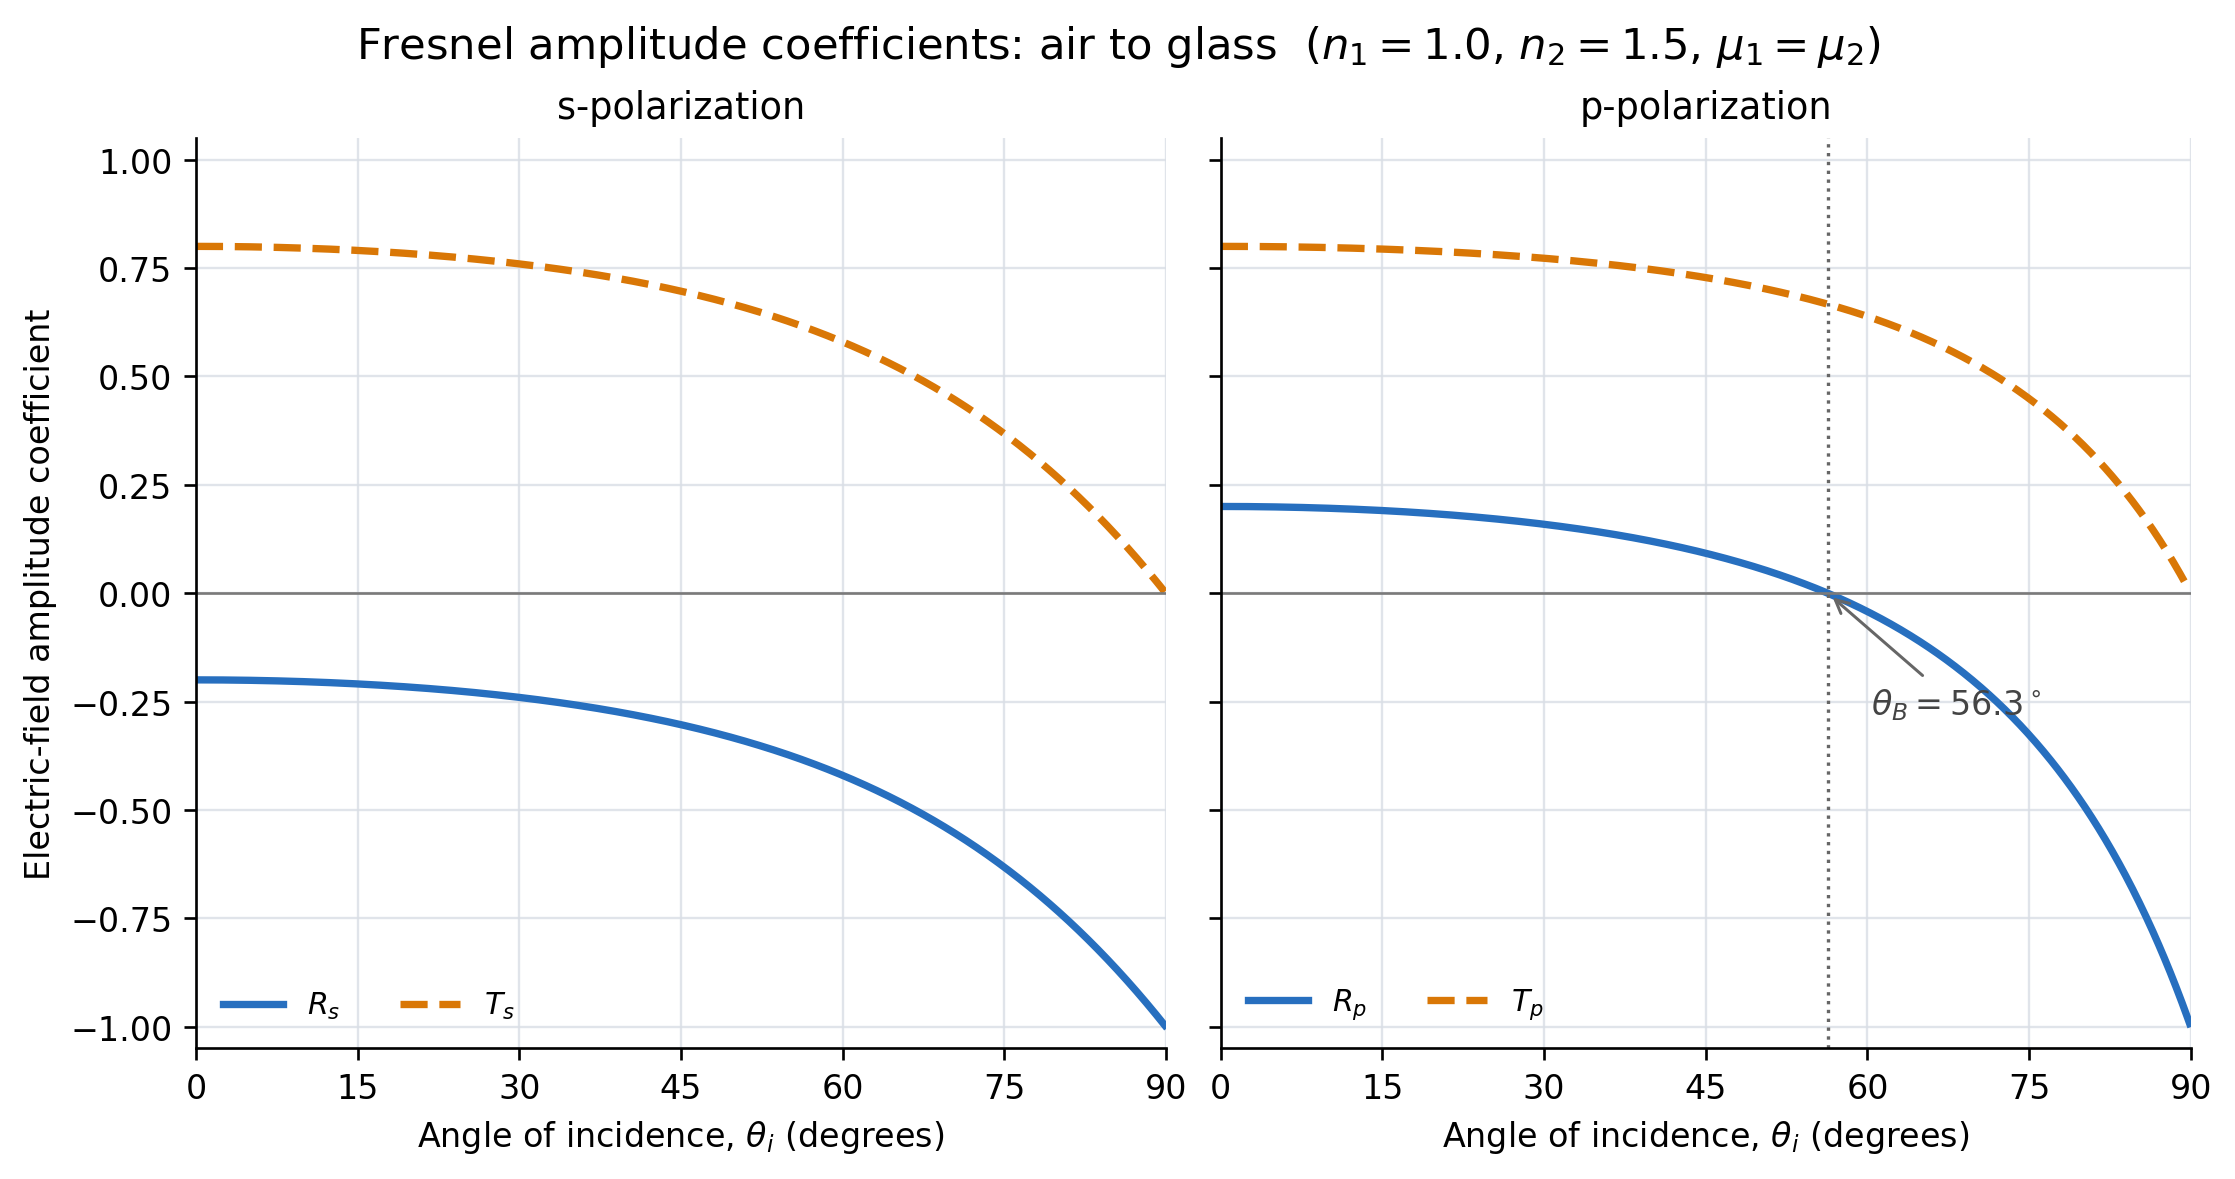
\includegraphics[width=0.85\textwidth]{images_reflection_refraction/fresnel.png}
    \caption{The fresnel coefficients for glass as a function of the incident angle. Note that for the \(p\)-polarised wave, there is a point where the reflected wave vanishes. That point is the \textsf{\textcolor{red!70!black}{brewster angle}}.}
\end{figure}
\begin{remark}
The labels \(s\) and \(p\) come from the German words
\textsf{senkrecht} (perpendicular) and \textsf{parallel}. The plane of
incidence is the plane containing the incident wave vector and the normal to
the interface; the reflected and transmitted wave vectors also lie in this
plane.

For \(s\)-polarized waves, the electric field is perpendicular to the plane of
incidence. For \(p\)-polarized waves, the electric field is parallel to the
plane of incidence.
\end{remark}

\subsection{The brewster angle}
The Brewster angle is the angle at which the
\textcolor{red!70!black}{\textsf{\(p\)-polarized reflection coefficient}}
vanishes. Setting the numerator of \(R_p\) to zero gives
\[
\eta_1\cos\theta_B=\eta_2\cos\theta_t,
\qquad
n_1\sin\theta_B=n_2\sin\theta_t.
\]
Eliminating \(\theta_t\) gives
\[
\tan^2\theta_B
=
\frac{(\eta_1^2-\eta_2^2)n_2^2}
     {\eta_2^2(n_2^2-n_1^2)}.
\]
For non-magnetic dielectrics, where \(\mu_1=\mu_2\), this simplifies to
\[
\theta_B=\arctan\left(\frac{n_2}{n_1}\right).
\]

\begin{theorem}[Brewster angle]
The Brewster angle \(\theta_B\) is the angle of incidence for which
\(R_p=0\). In general, for magnetic media,
\[
\tan^2\theta_B
=
\frac{(\eta_1^2-\eta_2^2)n_2^2}
     {\eta_2^2(n_2^2-n_1^2)}.
\]
For non-magnetic dielectrics, where \(\mu_1=\mu_2\), this simplifies to
\[
\tan\theta_B=\frac{n_2}{n_1}.
\]
\end{theorem}


\end{document}